%!TEX TS-program = xelatex
% Bu dosya sjuoz_word2latex.py tarafından otomatik üretildi.
\documentclass[9pt]{extarticle}
\usepackage{multicol}
\usepackage[top=0.5in, bottom=0.75in, right=0.75in, left=0.75in, headheight=0.25in, includehead]{geometry}
\usepackage{fontspec}
\usepackage{amsmath}
\usepackage{amssymb}
\usepackage{graphicx}
\usepackage{xcolor}
\usepackage{array}
\usepackage{tabularx}
\usepackage{booktabs}
\usepackage{multirow}
\usepackage{caption}
\usepackage{titlesec}
\usepackage{fancyhdr}
\usepackage{qrcode}
\usepackage{xurl}
\usepackage{lastpage}
\usepackage{indentfirst}
\usepackage{eso-pic}
\usepackage{tikz}
\usepackage[colorlinks=true, urlcolor=blue, linkcolor=black, citecolor=black]{hyperref}

\titleformat{\section}{\large\bfseries\centering}{\thesection.}{1.0em}{}
\titleformat{\subsection}{\large\bfseries}{\thesubsection.}{0.5em}{}
\titleformat{\subsubsection}{\normalsize\bfseries\itshape}{\thesubsubsection.}{0.5em}{}
\titlespacing*{\section}{0pt}{8pt}{6pt}
\titlespacing*{\subsection}{0pt}{8pt}{4pt}
\titlespacing*{\subsubsection}{0pt}{6pt}{3pt}

\newcommand{\titlesize}{\fontsize{12}{10}}
\renewcommand{\normalsize}{\fontsize{9pt}{9pt}\selectfont}
\renewcommand{\large}{\fontsize{10pt}{10pt}\selectfont}
\renewcommand{\small}{\fontsize{8pt}{8pt}\selectfont}
\captionsetup[table]{labelfont=bf, justification=raggedright, singlelinecheck=false}
\captionsetup[figure]{labelfont=bf, justification=centering, singlelinecheck=false}
\definecolor{sjuozblue}{HTML}{C1D1EB}
\definecolor{colorabs}{HTML}{E2EAF4}

% Yazı tipleri: Times New Roman / Garamond yoksa benzerleri kullanılır
\IfFontExistsTF{Times New Roman}{\setmainfont{Times New Roman}}{%
  \IfFontExistsTF{TeX Gyre Termes}{\setmainfont{TeX Gyre Termes}}{%
    \IfFontExistsTF{Liberation Serif}{\setmainfont{Liberation Serif}}{}}}
\IfFontExistsTF{Garamond}{\newfontfamily{\garamond}{Garamond}}{%
  \IfFontExistsTF{EB Garamond}{\newfontfamily{\garamond}{EB Garamond}}{\newcommand{\garamond}{\rmfamily}}}

\newcommand{\sjuozdoi}{https://doi.org/10.25271/sjuoz.2026.14.4.1993}
% İlk sayfadaki bilgi kutusunun sayfa altından yüksekliği ve metin için ayrılan boşluk
\newcommand{\firstfooterbottom}{0.4in}
\newcommand{\firstpagereserve}{1.4in}
% Sadece ilk sayfada metin alanını kısalt; ilk sayfa basıldıktan sonra eski haline döndür
\makeatletter
\newlength{\sjuozfulltextheight}
\AtBeginDocument{%
  \setlength{\sjuozfulltextheight}{\textheight}%
  \global\advance\textheight by -\firstpagereserve
  \global\@colht\textheight \global\@colroom\textheight \global\vsize\textheight
  \AddToHookNext{shipout/after}{\global\textheight\sjuozfulltextheight}}
\makeatother

% Başlık ve altlık (header/footer)
\pagestyle{fancy}
\fancyhf{}
\renewcommand{\headrulewidth}{0pt}
\lhead{\large \textit{Safi \textit{et al.}}}
\rhead{\small{\garamond{\textbf{SJUOZ|VOL14|OCT 2026|P571-\pageref*{LastPage}}}}}
\lfoot{\raisebox{8pt}{\textit{DOI:}\href{\sjuozdoi}{\textit{\small{\sjuozdoi}}}}}
\cfoot{\raisebox{8pt}{\thepage}}

\fancypagestyle{firstpage}{%
  \fancyhf{}
  \renewcommand{\headrulewidth}{0pt}
  \rhead{\IfFileExists{SJUOZ.png}{
\includegraphics[width=1.04in]{SJUOZ.png}}{\textbf{SJUOZ}}}
  \lhead{\colorbox{sjuozblue}{%
      \begin{minipage}[b]{0.83\textwidth}
        \vspace{0.15cm}
        \hspace{-3pt}\ \normalsize \noindent \garamond{Science Journal of University of Zakho}\\
        \normalsize \textit{\garamond{DOI: \sjuozdoi}}
        \vspace{0.2cm}
      \end{minipage}}}
}

% İlk sayfanın altındaki bilgi kutusu (sayfaya mutlak konumla yerleştirilir)
\newcommand{\sjuozfirstfooter}{%
  \begin{minipage}[b]{\textwidth}
      \rule{\textwidth}{1.5pt} \\[0.15cm]
      \begin{minipage}[t]{0.2\textwidth}\hspace{1pt} \small Access this article online \\
        \vspace{0.1cm}
        {\hypersetup{urlcolor=black}\qrcode[height=2.6162cm]{https://sjuoz.uoz.edu.krd/index.php/sjuoz/article/view/1993}}
      \end{minipage}\begin{minipage}[t]{0.4\textwidth}
        \small DOI:\href{\sjuozdoi}{\sjuozdoi} \\ \\[0.5cm]
        Printed ISSN 2663-628X; \\
        Electronic ISSN 2663-6298
      \end{minipage}\begin{minipage}[t]{0.4\textwidth}\small \textbf{Science Journal of University of Zakho} \\
        \textbf{Vol. 14, No. 04, pp. 571-\pageref*{LastPage}, October-2026} \\[0.5cm]
        This is an open access article under a CC BY-NC-SA 4.0 license \\
        (\href{https://creativecommons.org/licenses/by-nc-sa/4.0/}{https://creativecommons.org/licenses/by-nc-sa/4.0/})
      \end{minipage} \\[0.15cm]
      \rule{\textwidth}{1.5pt} \\[0.15cm]
      \centering \normalsize \thepage
  \end{minipage}}

% ORCID simgesi: orcid.png varsa o, yoksa çizilmiş yeşil "iD" simgesi
\definecolor{orcidgreen}{HTML}{A6CE39}
\newcommand{\orcidicon}{\IfFileExists{orcid.png}{
\includegraphics[width=9pt]{orcid.png}}{%
  \tikz[baseline=-0.7ex]{\fill[orcidgreen] (0,0) circle (4.5pt);
  \node[text=white, font=\fontsize{4.5pt}{4.5pt}\selectfont\bfseries, inner sep=0pt] at (0,0) {iD};}}}
\newcommand{\orcidlink}[1]{\href{#1}{\orcidicon}}

\begin{document}
\setcounter{page}{571}
\thispagestyle{firstpage}
\AddToShipoutPictureFG*{\put(\LenToUnit{0.75in},\LenToUnit{\firstfooterbottom}){\sjuozfirstfooter}}

\noindent \large \textbf{Original Article} \\[-5pt]
\begin{center} \titlesize \textbf{PERFORMANCE ENHANCEMENT FOR MOUTH DETECTION TIME BASED ON MODIFIED VIOLA-JONES ALGORITHM} \end{center}
\begin{center} \large \textbf{Mohammed E. Safi \textsuperscript{1,*}\orcidlink{https://orcid.org/0000-0003-4267-1702}, Eyad I. Abbas \textsuperscript{1}\orcidlink{https://orcid.org/0000-0002-5087-4713}, and Alaa H. Ali \textsuperscript{2}\orcidlink{https://orcid.org/0000-0002-6982-4994}}
\end{center}
\noindent
\large \textsuperscript{1}College of Electrical Engineering, University of Technology- Iraq, Baghdad, Iraq.\\
\large \textsuperscript{2}Department of Medical Instrumentation Techniques Engineering, Al-Mustaqbal University, 51001, Babylon, Iraq.\\

\begin{center} \textsuperscript{*}\textit{Corresponding author, E-mail:}\href{mailto:mohammed.e.safi@uotechnology.edu.iq}{mohammed.e.safi@uotechnology.edu.iq} (Tel: +964-7901848481)
\end{center}
\rule{\textwidth}{1.5pt}
\begin{minipage}[t]{0.175\textwidth}
  \hspace{0cm} \vspace{0cm}
\end{minipage} \begin{minipage}[t]{0.8\textwidth}
\large \textbf{ABSTRACT}\end{minipage} \\[-6pt]
\rule{\textwidth}{1.5pt} \\
\begin{minipage}[t]{0.175\textwidth}
  \vspace{1cm} Received \\ XX \\[0.5cm] Accepted \\ XX \\[0.5cm] Published \\ XX \\[0.25cm]
\end{minipage} \colorbox{colorabs}{\begin{minipage}[t]{0.81\textwidth}
  \large{Mouth detection is an important issue in visual speech recognition. The de facto algorithm used to achieve this is the Viola-Jones algorithm. Nevertheless, time enhancement for the auto-detection of this algorithm is required. Therefore, the goal of this research is to propose a modified approach based on the Viola-Jones algorithm to enhance the detection time. The main contribution of the proposed algorithm is limiting the auto-valuing for the threshold of the Viola-Jones algorithm and enhancing the time by configuring the maximum step for the adaptive threshold value. The UOTletters database was used in the experiments of this research with 30 speakers pronouncing English letters with overall frames of 28164. The experiment results have shown that the average detection time for the proposed method was 0.585 sec, compared with the baseline method's 2.097 sec. As a result, the proposed approach enhanced the mouth detection time with respect to the baseline algorithm (358.46\%). Consequently, the proposed algorithm is a good solution for real-time visual speech recognition regarding the detection time enhancement.
  \\[2pt]
  \normalsize \textbf{Keywords:} Mouth detection; Viola-Jones algorithm; adaptive threshold value.
  }
\end{minipage}}
\\[-10pt]

\normalsize
\noindent \rule{\textwidth}{0.75pt}
\begin{multicols}{2}
\section{INTRODUCTION}
Machine learning is witnessing a rise in many applications in communications, enabling smarter resource allocation, enhanced signal processing, and more adaptive algorithms (Radhi \textit{et al.}, 2022). Speech recognition nowadays has become one of the most common features in many applications and devices (Mohammed E. Safi \& Abbas, 2016). Nevertheless, the challenge of enhancing accuracy in audio speech recognition is required (Mohammed Ehsan Safi \& Abbas, 2022). As a result, visual speech recognition was adopted to assist audio speech recognition. Visual speech recognition, basically in common algorithms, consists of three parts: Mouth detection, lips isolation, and finally classification (Mohammed Ehsan Safi \& Abbas, 2023). Mouth detection is a machine-learning process that is used to detect the human mouth and separate it from its surroundings (Kaur \& Sharma, 2017). Many approaches are used in this field, as shown in research (Balasubramanian \textit{et al.}, 2009; Nguyen \textit{et al.}, 2006; Ryu \& Oh, 2001), but the Viola-Jones algorithm became a de facto algorithm (Wisam H Ali \textit{et al.}, 2020; Ibrahim \& Mulvaney, 2015; Viola \& Jones, 2001). The Viola-Jones algorithm (VJA) is a machine-learning algorithm for detecting and analyzing Human face parts from images with high speed and accuracy (Maghraby \textit{et al.}, 2014). VJA in color images is converted to grayscale. Therefore, in Haar-like features, it's important to specify the threshold for it to configure edges. The thresholds in some pieces of research are static thresholds, such as (Wisam H Ali \textit{et al.}, 2020; Setu \& Rahman, 2016). In research (Joshi \textit{et al.}, 2021), the optimal threshold for mouth detection was studied. The experiment results of this study have shown that the maximum accuracy at the threshold value of 150, by accuracy of 73.07\% and 92.30\%, respectively. The database was selected at 5ft and 8ft distance respectively. In practical and real-time videos, not all frames have the same threshold due to differences in environments like illumination and skin color. As a result, auto-configuring to the optimal threshold was proposed by (Indrabayu \textit{et al.}, 2019). They suggested a modification for VJA by using a zero value as the initial for the threshold parameter. The auto-valuing threshold 938 face frames for 20 videos yields 5.665 sec. in mouth detection feature time with an accuracy of 99.49\%. In this paper, a modification Viola-Jones algorithm using an adaptive threshold for optimized algorithms (Indrabayu \textit{et al.}, 2019) and (Joshi \textit{et al.}, 2021), respectively, was proposed. The drawbacks of the previous works based on a fixed threshold value are problems related to moving objects and varying light and distance. The drawback of the baseline auto-valuing threshold is that it is time-consuming because the criteria determination is based on practical observation only and is not supported by analytical calculations.

The main contribution of the proposed algorithm is limiting the auto-valuing of the threshold of the Viola-Jones algorithm and reducing the time by configuring the maximum step for the adaptive threshold value. The selection of the search step was improved by analyzing the group of threshold values using polynomial curve fitting of the linear equation. Moreover, the direction of the adaptive threshold value step (increment or decrement) was determined based on experimental results and analytical determination. The experiment results were performed on the UOTletters database (Wisam H Ali \textit{et al.}, 2020), which consists of 30 speakers pronouncing English letters with overall frames of 28164.

\end{multicols}
\noindent
\begin{minipage}{\textwidth}
\centering
\captionof{table}{Related works' drawbacks.}
\vspace{-6pt}
\small
\begin{tabularx}{\textwidth}{@{}>{\raggedright\arraybackslash}X>{\raggedright\arraybackslash}X>{\raggedright\arraybackslash}X>{\raggedright\arraybackslash}X@{}}
\toprule
\textbf{Reference} & \textbf{Algorithm} & \textbf{Threshold} & \textbf{Drawback} \\ \midrule
(Wisam H Ali \textit{et al.}, 2020; Ibrahim \& Mulvaney, 2015; Viola \& Jones, 2001) & Standard Viola \& Jones algorithm & Static, based on distance and light contrast & Misses detection with varying light and distance \\ \addlinespace[0.3em]
(Joshi \textit{et al.}, 2021) & Standard Viola \& Jones algorithm with a fixed threshold based on distance & The threshold value is 150 at 5 ft and 8 ft distances, respectively & Miss detection with varying light and distance more than 8 ft distances and less 5 ft. \\ \addlinespace[0.3em]
(Indrabayu \textit{et al.}, 2019) & Modified Viola \& Jones algorithm & Auto-valuing for Threshold starting from 1 to unlimited value & Cost of time and cause of error if no object detection. \\ \addlinespace[0.3em]
(Joshi \textit{et al.}, 2021) & Modified Viola \& Jones algorithm & Auto-valuing for Threshold starting from 1 to unlimited value maximum values of 150 at 3 ft to 8 ft of distance & Cost of time. \\ \addlinespace[0.3em]
The proposed algorithm & The proposed Modified Viola \& Jones algorithm & Auto Valuing for Threshold starting from 150 to 1 at 3 ft to 8 ft of distance & Starting value for distance more than 8 ft. (Future works) \\
\bottomrule
\end{tabularx}
\end{minipage}
\par\vspace{6pt}

\begin{multicols}{2}
\section{VIOLA-JONES ALGORITHM}
VJA has many features, like dealing with different skin colors, the ability to detect even with eyeglasses, and the ability to recognize many faces in one image (Zhang \& Zhang, 2010). The algorithm is based on rectangular-shaped features called Haar-Like features (Papageorgiou \textit{et al.}, 1998). This feature distinguishes the boundaries of the faces from their surroundings in the frame. This technique is effective even for different face images with different ranges. The algorithm with features is faster than the algorithm that works on a pixel operation. As a result, employing characteristics of pictures is used more than pixel-based ones (Wissam Hassan Ali, 2016). Figure 1 illustrates most shapes of rectangle features, which consist of a white pixel area and a black pixel area (Indrabayu \textit{et al.}, 2019). The concept of using Haar-like features is to follow the boundaries of objects by subtracting the white area from the black area:

\begin{equation}
  V = \sum P_{(\mathit{white}\ \mathit{region})} - \sum P_{(\mathit{black}\ \mathit{region})}
\end{equation}
Where: P is the value of the pixel, and V is the feature value.

\noindent\begin{minipage}{\linewidth}
\centering
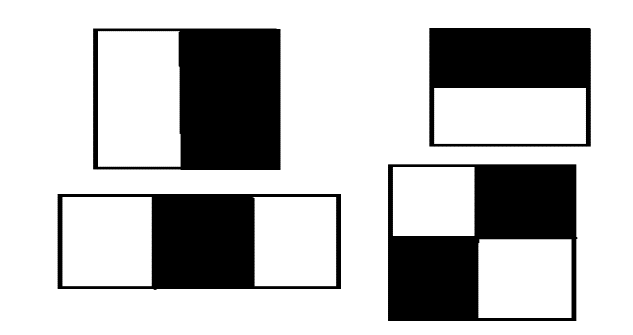
\includegraphics[width=\linewidth, height=0.42\textheight, keepaspectratio]{Figure1.png}
\captionof{figure}{Different shapes of Haar-like features.}
\end{minipage}
\par\vspace{6pt}

To minimize the complexity of the mathematical operations, the Viola-Jones algorithm converts the input image into grayscale and into a new mathematical form called the integral image to minimize the calculation time. The integral image is determined by the sum of the upper rectangle for the current pixel (Kherchaoui \& Houacine, 2010):

\begin{equation}
  \mathit{In}_{\left( i,j \right)}=\sum\limits_{\bar{i}=1,\bar{j}=1}^{i-1,j-1} \mathit{Image}(\bar{i},\bar{j})
\end{equation}
Where: In is the integral image, Image is the input image, and (i,j) is the spatial pixel at the x and y coordinates, respectively.

The integral image is determined by taking the spatial value of the bottom-left pixel of the feature window and subtracting the remaining unwanted region of the integral image to obtain the contrast of the Haar-like features, which leads to decreased detection time. For example, as shown in Figure 2, two areas of Haar’s feature window represent the cases of calculation for areas in the integral image (Berbar \textit{et al.}, 2006).

\noindent\begin{minipage}{\linewidth}
\centering
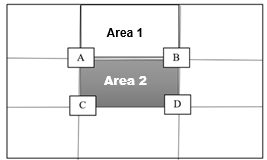
\includegraphics[width=\linewidth, height=0.42\textheight, keepaspectratio]{Figure2.png}
\captionof{figure}{Integral image example.}
\end{minipage}
\par\vspace{6pt}

The two cases are the region with an edge surrounding it and the region with an unwanted area boundary. The edge surrounding the Area illustrated in Area 1 of Figure 2 can be calculated as given below:

\begin{equation}
  v_{1}=B-A
\end{equation}
The Area with unwanted Areas surrounding it, illustrated in Area 2 of Figure 2, can be calculated as given below:

\begin{equation}
  v_{2}=D-\left( B+C \right)+A
\end{equation}
It is obvious that point A is added because it is subtracted twice from point D (point A is compact with points B and C in the undesired areas). In the same example in Figure 2, it could estimate the Haar-like feature value by subtracting v1 from v2 using the same principle of Equation 1.

VJA has another concept to reduce the massive number of features; eg., a 24*24 window gives 160,000 features. Viola and Jones proposed two techniques to overcome this problem: using a cascade filter and AdaBoost training, as shown in Figure 3. Some of the obtained features are not useful for face detection. Therefore, a cascade filter was utilized to crumble the detection operation of faces into substages like eyes, nose bridge, and mouth region. In addition, to build a strong classifier, the subsequent weak classifier corrected the error in the previous classifier by AdaBoost training (Setu \& Rahman, 2016).

\noindent\begin{minipage}{\linewidth}
\centering
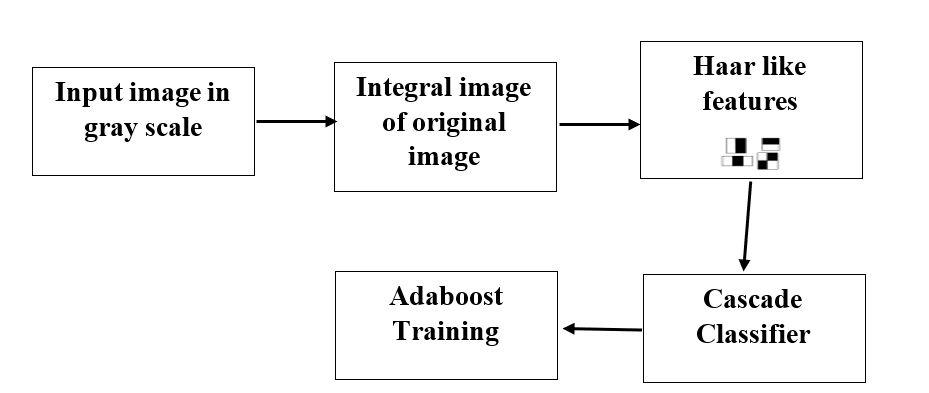
\includegraphics[width=\linewidth, height=0.42\textheight, keepaspectratio]{Figure3.png}
\captionof{figure}{Viola and Jones algorithm.}
\end{minipage}
\par\vspace{6pt}

The final results of detection for the images that have multi-candidate detection are surrounded by merging the bounding boxes around the targets. The configuration step of the threshold governs the grouping of the collocated detection boxes. The selection of the optimal merged bounding box threshold would correctly overcome error type 1 (false positive) and time delay or error type 2 (miss detection). The effect of the minimum value of the threshold which led to a false positive illustrated in Figure 4. Nevertheless, error type 2 could occur due to an increase in the threshold (Joshi \textit{et al.}, 2021). Consequently, that parameter is a tunable value in the function (vision.CascadeObjectDetector) in MATLAB (MathWorks, n.d.).

\noindent\begin{minipage}{\linewidth}
\centering
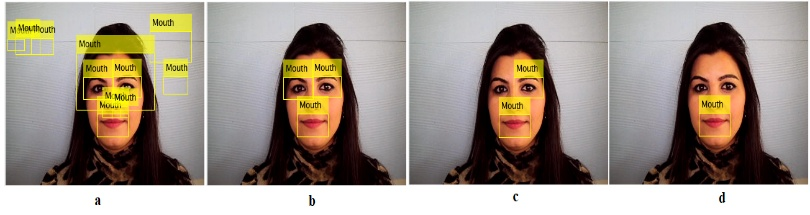
\includegraphics[width=\linewidth, height=0.42\textheight, keepaspectratio]{Figure4.jpeg}
\captionof{figure}{(a). Detection when Threshold=1 (b). Detection when Threshold = 10 (c). Detection when Threshold =80 (d). Detection when Threshold =90.}
\end{minipage}
\par\vspace{6pt}

\section{PROPOSED MOUTH DETECTION ALGORITHM}
The proposed algorithm is inspired by the adaptive value of the algorithm proposed in (Indrabayu \textit{et al.}, 2019). Yet, the selection of the auto-valuing of the optimal threshold is the opposite way. Moreover, the proposed algorithm adopts a technique to maximize the search step.

Figure 5 shows the proposed algorithm procedure; the starting point for the threshold is 150 instead of one initial value in the study (Indrabayu \textit{et al.}, 2019), due to our observation in Section 4 that most values of the optimal threshold are in the upper limit. Moreover, the selection of the upper limit of the optimal threshold (150) is based on observations in the study (Joshi \textit{et al.}, 2021) and our practical experiments for the maximum value that the threshold values reached. In addition, another contribution of the proposed algorithm is to select the search step, which is set to 5. Consequently, the adaptive threshold value (TH) is decreased by (5) until reaching the ROI or reaching the last value (1):

\begin{equation}
  \mathit{TH}_{t}= \mathit{TH}_{t-1}-5
\end{equation}
Equation 5 is determined based on analytic and experimental results in Section 4.

\noindent\begin{minipage}{\linewidth}
\centering
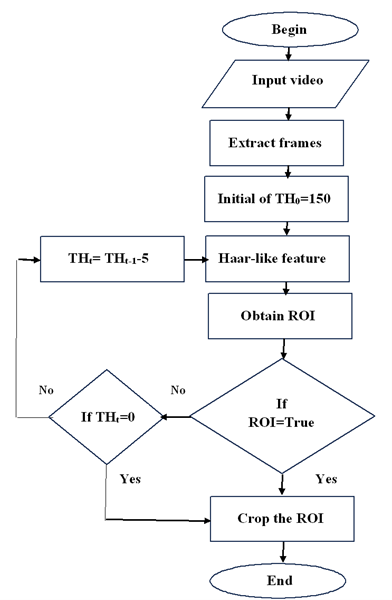
\includegraphics[width=\linewidth, height=0.42\textheight, keepaspectratio]{Figure5.png}
\captionof{figure}{The proposed adaptive algorithm of the optimal threshold for mouth detection.}
\end{minipage}
\par\vspace{6pt}

\section{EXPERIMENTAL RESULTS}
Figure 6 shows sample images of faces and the detected mouth using the proposed algorithm for the UOTletters database. In this section, many experiments were done to ensure that the analytical results satisfy the practical results. Moreover, make an overall evaluation of the proposed algorithm with respect to the baseline algorithm for the thirty speakers pronouncing English letters, with overall frames 28164. Equation 5 is determined from the curve fitting for the threshold based on the detection results, in addition to the distribution of the detection results. As we can see in Figure 7, the sample values of the threshold for the letter A for thirty speakers are most of the values located in the upper area for the proposed range (1 to 150). Consequently, we proposed starting at 150 and then decreasing the threshold value to adopt the optimal value instead of the increment approach in the baseline algorithm. Moreover, the selection of the search step was improved by analyzing the group of threshold values using polynomial curve fitting of the linear equation:

\begin{equation}
  \mathit{TH}_{t}= {a\ \mathit{TH}}_{t-1}+b
\end{equation}
Where THt is the predicted value of the threshold, and THt-1 is the previous value of it.

Practically, the two coefficients, a and b, are limited to integer values due to the threshold criteria, in addition to the detection ratio.

\noindent\begin{minipage}{\linewidth}
\centering
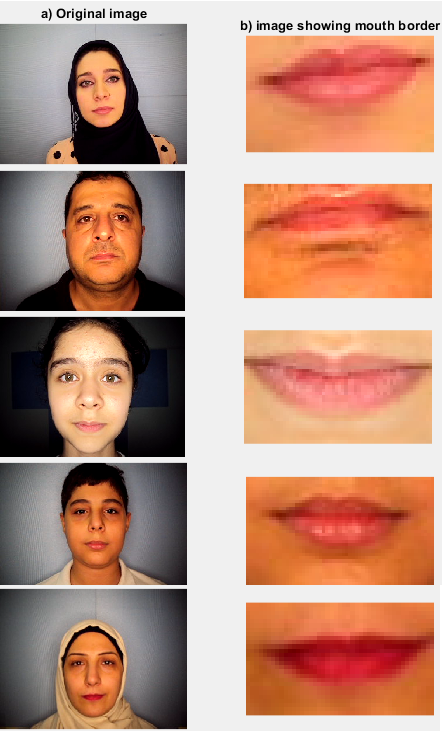
\includegraphics[width=\linewidth, height=0.42\textheight, keepaspectratio]{Figure6.png}
\captionof{figure}{Sample images of faces and the detected mouth using the proposed algorithm for the UOTletters database.}
\end{minipage}
\par\vspace{6pt}

As shown in Figure 8, using the analytic polynomial curve fitting between TH\textsubscript{t} and TH\textsubscript{t-1}, the value of the (a) coefficient was determined (0.909). Yet, the (a) value must be an integer value due to the threshold criteria; therefore, it is approximated to (1). While the (b) value is analytically (10.4), and in the same manner, its value is approximated to (10) due to the threshold criteria. The reason for applying the analytic step is to calculate the maximum searching step (represented by the b coefficient) for the threshold value and specify the framework for the practical experiment to select the final value of the optimal searching step.

\noindent\begin{minipage}{\linewidth}
\centering
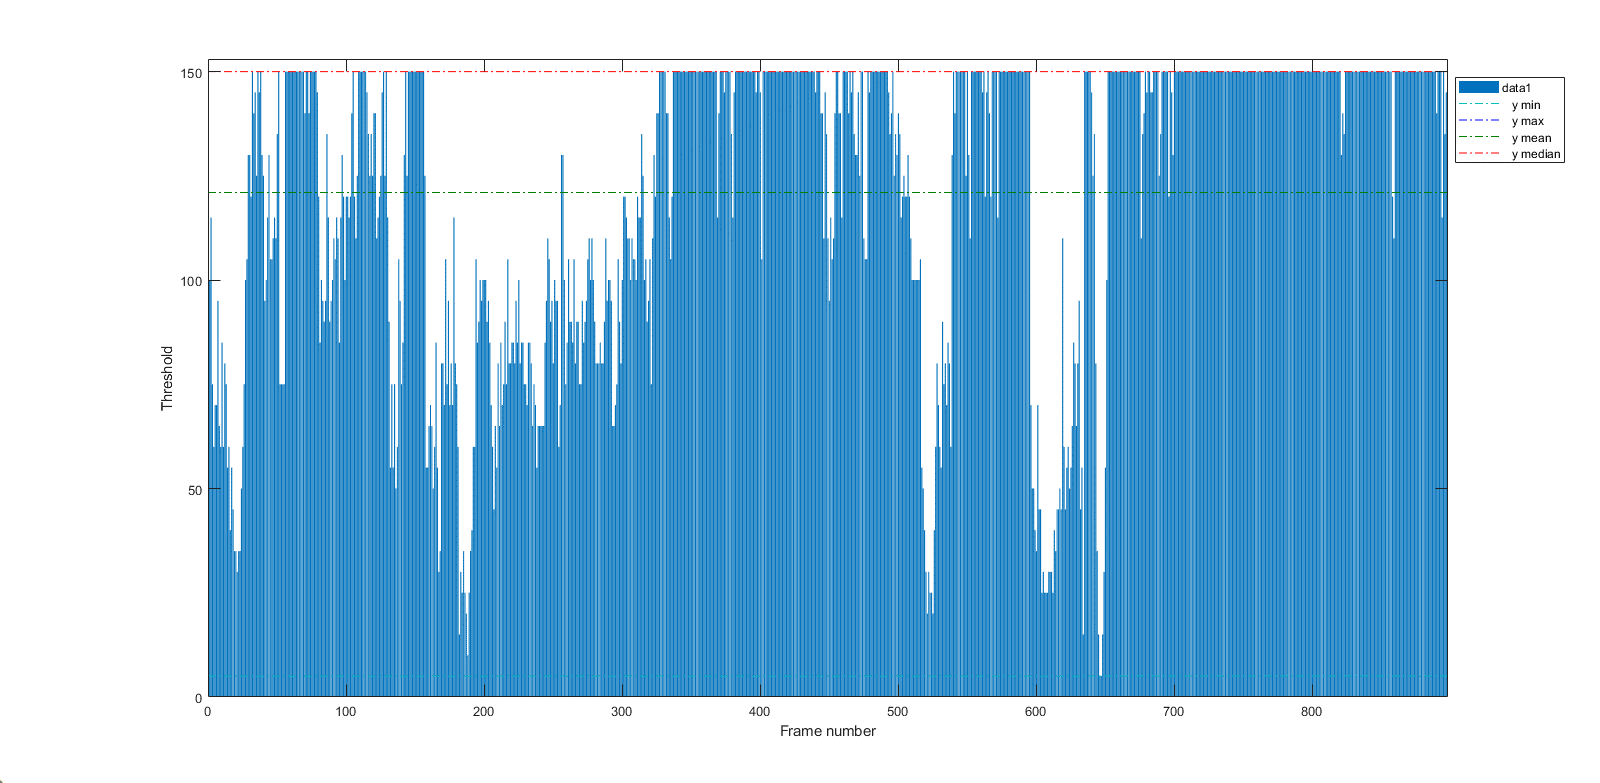
\includegraphics[width=\linewidth, height=0.42\textheight, keepaspectratio]{Figure7.png}
\captionof{figure}{Sample values of the threshold for the letter A for thirty speakers.}
\end{minipage}
\par\vspace{6pt}

For the second criterion (detection ratio), a practical experiment for accuracy versus values of the searching step was applied to examine the b coefficient values (1 to 10). As shown in Figure 9, the maximum searching step with the highest accuracy is (5).

\noindent\begin{minipage}{\linewidth}
\centering
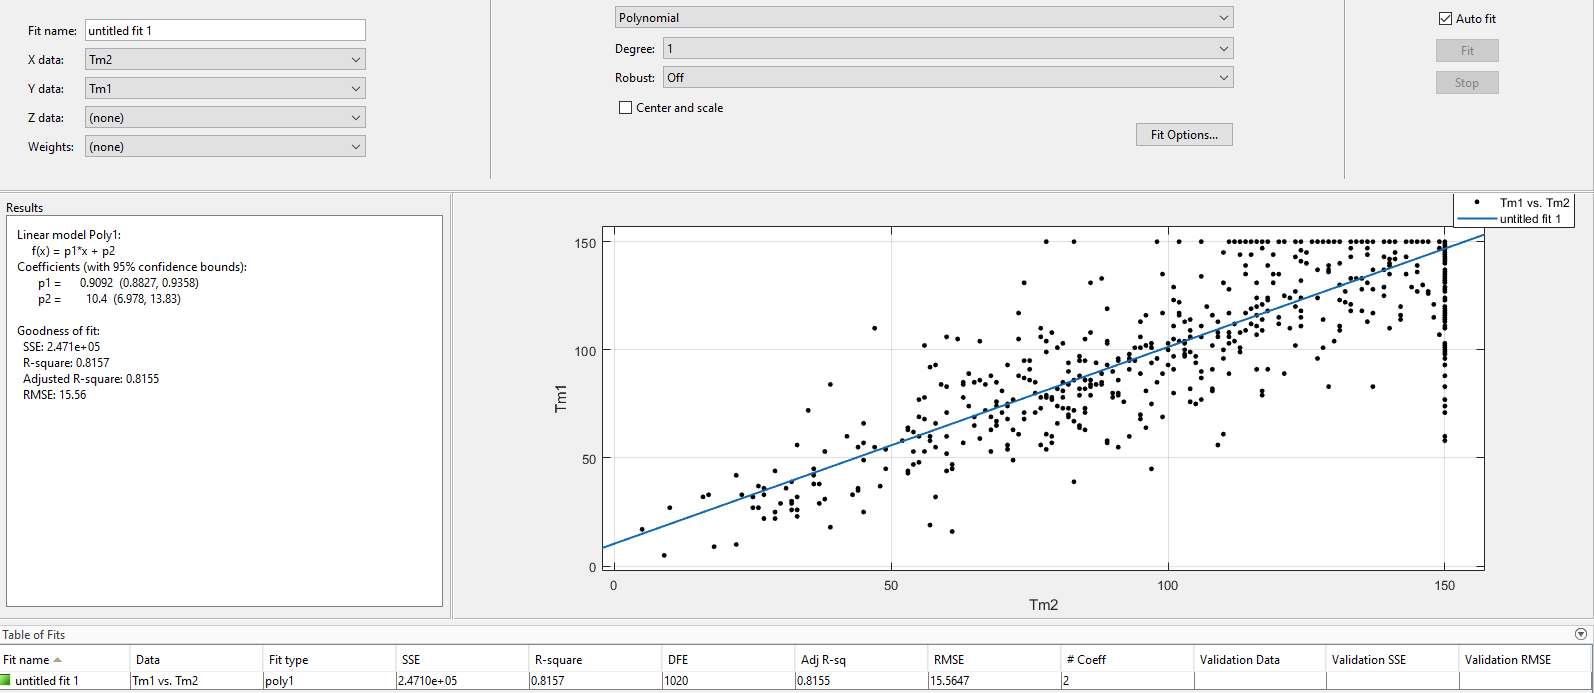
\includegraphics[width=\linewidth, height=0.42\textheight, keepaspectratio]{Figure8.png}
\captionof{figure}{The curve fitting for TH\textsubscript{t} (Tm1) versus TH\textsubscript{t-1} (Tm2).}
\end{minipage}
\par\vspace{6pt}

\noindent\begin{minipage}{\linewidth}
\centering
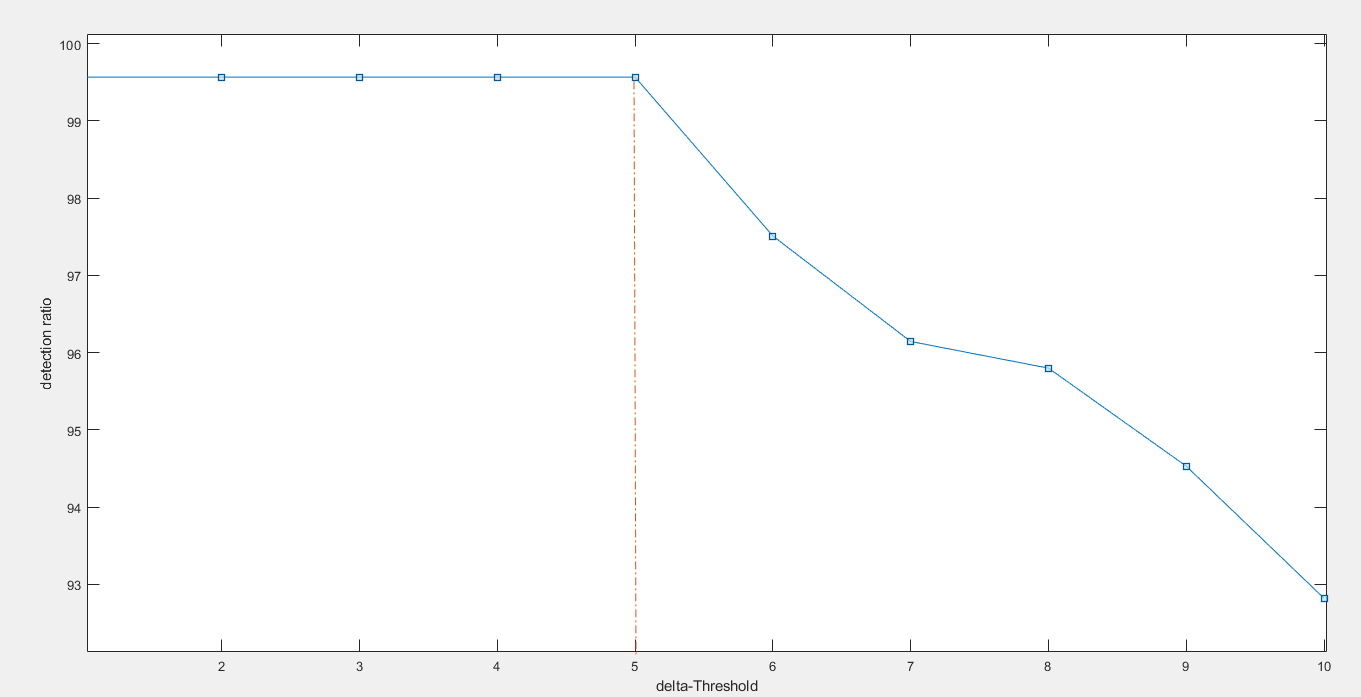
\includegraphics[width=\linewidth, height=0.42\textheight, keepaspectratio]{Figure9.png}
\captionof{figure}{Accuracy versus (b coefficient).}
\end{minipage}
\par\vspace{6pt}

The final experiment evaluation based on accuracy and time delay with respect to the baseline algorithm (Indrabayu \textit{et al.}, 2019) was illustrated in Table 1. The experiment results show that the baseline algorithm has an accuracy of 99.567\% with an average detection time (TD) of 2.097 s. Nevertheless, the proposed algorithm has the same accuracy of 99.567\% with an average detection time (TD) of 0.585 sec.). Consequently, the proposed algorithm has sped up the calculation process by 3.5846 times that of the baseline algorithm.

The drawback of this study is that the experimental results are limited to a maximum distance of 8 ft from the camera; therefore, the maximum limit (150) may change at greater distances depending on the application and real-time implementation.

\end{multicols}
\noindent
\begin{minipage}{\textwidth}
\centering
\captionof{table}{Evaluation of the proposed and baseline methods.}
\vspace{-6pt}
\footnotesize
\begin{tabularx}{\textwidth}{@{}>{\raggedright\arraybackslash}X>{\centering\arraybackslash}X>{\centering\arraybackslash}X>{\centering\arraybackslash}X>{\centering\arraybackslash}X>{\centering\arraybackslash}X>{\centering\arraybackslash}X@{}}
\toprule
\textbf{No. of speakers} & \textbf{No. of frames} & \textbf{Detected} & \textbf{Accuracy (\%)} & \textbf{Average thresholds} & \textbf{average T\textsubscript{D} (Sec.) (Indrabayu \textit{et al.}, 2019)} & \textbf{The proposed method's average T\textsubscript{D} (Sec.)} \\ \midrule
1 & 1019 & 1019 & 100 & 144 & 4.126 & 0.1748 \\ \addlinespace[0.3em]
2 & 985 & 985 & 100 & 137 & 0.068 & 0.9864 \\ \addlinespace[0.3em]
3 & 1057 & 1057 & 100 & 40 & 3.97 & 0.206 \\ \addlinespace[0.3em]
4 & 1161 & 1160 & 99.9 & 130 & 3.94 & 0.212 \\ \addlinespace[0.3em]
5 & 962 & 953 & 99.1 & 45 & 0.15 & 1.03 \\ \addlinespace[0.3em]
6 & 786 & 786 & 100 & 142 & 4.33 & 0.134 \\ \addlinespace[0.3em]
7 & 992 & 992 & 100 & 135 & 2.77 & 0.446 \\ \addlinespace[0.3em]
8 & 785 & 785 & 100 & 66 & 0.665 & 0.867 \\ \addlinespace[0.3em]
9 & 803 & 803 & 100 & 120 & 2.87 & 0.426 \\ \addlinespace[0.3em]
10 & 896 & 896 & 100 & 129 & 3.34 & 0.332 \\ \addlinespace[0.3em]
11 & 898 & 898 & 100 & 140 & 3.86 & 0.228 \\ \addlinespace[0.3em]
12 & 819 & 819 & 100 & 144 & 3.835 & 0.233 \\ \addlinespace[0.3em]
13 & 841 & 841 & 100 & 126 & 1.91 & 0.618 \\ \addlinespace[0.3em]
14 & 794 & 794 & 100 & 91 & 1.55 & 0.69 \\ \addlinespace[0.3em]
15 & 788 & 788 & 100 & 77 & 1.025 & 0.795 \\ \addlinespace[0.3em]
16 & 771 & 771 & 100 & 90 & 1.03 & 0.794 \\ \addlinespace[0.3em]
17 & 889 & 889 & 100 & 91 & 0.18 & 1.001 \\ \addlinespace[0.3em]
18 & 945 & 945 & 100 & 135 & 3.515 & 0.297 \\ \addlinespace[0.3em]
19 & 992 & 992 & 100 & 113 & 2.5515 & 0.489 \\ \addlinespace[0.3em]
20 & 957 & 957 & 100 & 105 & 1.575 & 0.685 \\ \addlinespace[0.3em]
21 & 867 & 867 & 100 & 129 & 2.13 & 0.574 \\ \addlinespace[0.3em]
22 & 908 & 908 & 100 & 75 & 0.29 & 0.942 \\ \addlinespace[0.3em]
23 & 932 & 932 & 100 & 134 & 0.56 & 0.888 \\ \addlinespace[0.3em]
24 & 965 & 965 & 100 & 107 & 2.155 & 0.569 \\ \addlinespace[0.3em]
25 & 973 & 973 & 100 & 138 & 2.205 & 0.559 \\ \addlinespace[0.3em]
26 & 1018 & 1018 & 100 & 145 & 3.025 & 0.395 \\ \addlinespace[0.3em]
27 & 1010 & 1010 & 100 & 121 & 0.58 & 0.539 \\ \addlinespace[0.3em]
28 & 1223 & 1150 & 94 & 85 & 0.58 & 0.884 \\ \addlinespace[0.3em]
29 & 1045 & 1045 & 100 & 145 & 0.12 & 1.024 \\ \addlinespace[0.3em]
30 & 870 & 870 & 100 & 144 & 4.015 & 0.197 \\ \addlinespace[0.3em]
Overall & 28164 & 28008 & 99.567 & 114 & 2.097 & 0.585 \\
\bottomrule
\end{tabularx}
\end{minipage}
\par\vspace{6pt}

\begin{multicols}{2}
\section{CONCLUSIONS}
The mouth detection time is an important issue in visual speech recognition. In this paper, a modification of VJA using an adaptive threshold was proposed. The experimental results have shown that our algorithm enhanced the mouth detection time with the baseline algorithm reduced to more than 3.5 times approximately. Consequently, the proposed algorithm gives a good solution for real-time visual speech recognition regarding the detection time enhancement. The drawback of this paper is that the experimental results are limited to a maximum distance of 8 ft from the camera; therefore, the maximum limit (150) may change at greater distances depending on the application and real-time implementation. Moreover, the limitation of the present study is an important direction for future validation using more diverse datasets.

\subsection*{ACKNOWLEDGEMENTS}
\textbf{“The authors sincerely thank the original investigators,} \textbf{Wisam H Ali, R. Saeed, and H. Al-Muifraje, for their foundational work and for making the dataset from their published study} (Wisam H Ali \textit{et al.}, 2020) \textbf{available for this retrospective analysis.”}

\subsection*{Ethical Statement}
\textbf{"The original data collection was conducted by the primary investigators} (Wisam H Ali \textit{et al.}, 2020) \textbf{with the official approval of their institutional university authorities at that time. Informed consent was explicitly obtained from all human volunteers by the original research team. For the present study, a secondary analysis was performed using this existing dataset, which was provided in a fully anonymized and de-identified format to protect participant confidentiality."}

\subsection*{Author Contributions}
\noindent Study concept and design: M. E. Safi, E. I. Abbas, A. H. Ali; Analysis and interpretation of data: M. E. Safi, E. I. Abbas; Drafting of the manuscript: M. E. Safi, E. I. Abbas, A. H. Ali; Critical revision of the manuscript for important intellectual content: M. E. Safi, E. I. Abbas; Statistical analysis: M. E. Safi, E. I. Abbas, A. H. Ali; Administrative, technical, and material support: M. E. Safi, E. I. Abbas, A. H. Ali; Study supervision: M. E. Safi, E. I. Abbas, A. H. Ali.

\subsection*{Conflict of Interest}
“The authors declare that they have no conflicts of interest related to the publication or funding of this manuscript.”

\subsection*{Funding}
“The authors declare that no financial support, grants, or funding were received from any public, commercial, or non-profit organizations for the research, authorship, or publication of this article.”

\section*{REFERENCES}
\begin{list}{}{
    \setlength{\leftmargin}{1.5em}
    \setlength{\itemindent}{-1.5em}
    \setlength{\parsep}{0pt}
    \setlength{\itemsep}{6pt}
}
\item Ali, Wisam H, R. Saeed, T., \& H. Al-Muifraje, M. (2020). FPGA Implementation of Visual Speech Recognition System based on NVGRAM-WNN. \textit{2020 International Conference on Computer Science and Software Engineering (CSASE)}, 132–137. DOI:\href{https://doi.org/10.1109/CSASE48920.2020.9142095}{https://doi.org/10.1109/CSASE48920.2020.9142095}

\item Ali, Wissam Hassan. (2016). \textit{Pattern Recognition System for Human Utterance} (Issue June). University of Technology-Iraq.

\item Balasubramanian, M., Palanivel, S., \& Ramalingam, V. (2009). Real time face and mouth recognition using radial basis function neural networks. \textit{Expert Systems with Applications}, \textit{36}(3, Part 2), 6879–6888. DOI:\href{https://doi.org/10.1016/j.eswa.2008.08.001}{https://doi.org/10.1016/j.eswa.2008.08.001}

\item Berbar, M. A., Kelash, H. M., \& Kandeel, A. A. (2006). Faces and Facial Features Detection in Color Images. \textit{Geometric Modeling and Imaging--New Trends (GMAI’06)}, 209–214. DOI:\href{https://doi.org/10.1109/GMAI.2006.18}{https://doi.org/10.1109/GMAI.2006.18}

\item Ibrahim, M. Z., \& Mulvaney, D. J. (2015). Geometrical-based lip-reading using template probabilistic multi-dimension dynamic time warping. \textit{Journal of Visual Communication and Image Representation}, \textit{30}, 219–233. DOI:\href{https://doi.org/10.1016/j.jvcir.2015.04.013}{https://doi.org/10.1016/j.jvcir.2015.04.013}

\item Indrabayu, Hasanuddin, \& Nurtanio, I. (2019). An Approach in Auto Valuing for Optimal Threshold of Viola Jones. \textit{Symposium of Emerging Nuclear Technology and Engineering Novelty}. DOI:\href{https://doi.org/10.1088/1742-6596/1198/9/092003}{https://doi.org/10.1088/1742-6596/1198/9/092003}

\item Joshi, A., Chavan, V., \& Kaveri, P. (2021). Semantic Gap Reduction From Mouth Feature Threshold Value Using Viola Jones Algorithm. \textit{ICCRDA 2020}. DOI:\href{https://doi.org/10.1088/1757-899X/1022/1/012065}{https://doi.org/10.1088/1757-899X/1022/1/012065}

\item Kaur, J., \& Sharma, A. (2017). Performance Analysis of Face Detection by using Viola-Jones algorithm. \textit{International Journal of Computational Intelligence Research}, \textit{13}(5), 707–717.

\item Kherchaoui, S., \& Houacine, A. (2010). Face detection based on a model of the skin color with constraints and template matching. \textit{2010 International Conference on Machine and Web Intelligence}, 469–472. DOI:\href{https://doi.org/10.1109/ICMWI.2010.5648043}{https://doi.org/10.1109/ICMWI.2010.5648043}

\item Maghraby, A. El, Abdalla, M., \& El, M. Y. (2014). Detect and Analyze Face Parts Information using Viola- Jones and Geometric Approaches. \textit{International Journal of Computer Applications}, \textit{101}(3), 23–28. DOI:\href{https://doi.org/10.5120/17667-8494}{https://doi.org/10.5120/17667-8494}

\item MathWorks. (n.d.). \textit{vision.CascadeObjectDetector (Detect objects using the Viola-Jones algorithm)}. Retrieved December 27, 2022, from \url{https://www.mathworks.com/help/vision/ref/vision.cascadeobjectdetector-system-object.html}

\item Nguyen, D., Halupka, D., Member, S., Aarabi, P., Sheikholeslami, A., \& Member, S. (2006). Real-Time Face Detection and Lip Feature Extraction Using Field-Programmable Gate Arrays. \textit{IEEE Transactions on Systems, Man, and Cybernetics}, \textit{36}(4), 902–912. DOI:\href{https://doi.org/10.1109/TSMCB.2005.862728}{https://doi.org/10.1109/TSMCB.2005.862728}

\item Papageorgiou, C. P., Oren, M., \& Poggio, T. (1998). A general framework for object detection. \textit{Sixth International Conference on Computer Vision (IEEE Cat. No.98CH36271)}, 555–562. DOI:\href{https://doi.org/10.1109/ICCV.1998.710772}{https://doi.org/10.1109/ICCV.1998.710772}

\item Radhi, A. A., Akkar, H. A. R., \& Abdullah, H. N. (2022). Skewness and access kurtosis as denoised mixed features-based K-Medoids for cooperative spectrum sensing. \textit{Physical Communication}, \textit{54}, 101831. DOI:\href{https://doi.org/10.1016/j.phycom.2022.101831}{https://doi.org/10.1016/j.phycom.2022.101831}

\item Ryu, Y.-S., \& Oh, S.-Y. (2001). Automatic extraction of eye and mouth fields from a face image using eigenfeatures and multilayer perceptrons. \textit{Pattern Recognition}, \textit{34}(12), 2459–2466. DOI:\href{https://doi.org/10.1016/S0031-3203(00)00173-4}{https://doi.org/10.1016/S0031-3203(00)00173-4}

\item Safi, Mohammed E., \& Abbas, E. I. (2016). Microcontroller - Controlled security door based on speech recognition. In \textit{Al-Sadiq International Conference on Multidisciplinary in IT and Communication Techniques Science and Applications, AIC-MITCSA 2016} (pp. 48–53). DOI:\href{https://doi.org/10.1109/AIC-MITCSA.2016.7759909}{https://doi.org/10.1109/AIC-MITCSA.2016.7759909}

\item Safi, Mohammed Ehsan, \& Abbas, E. I. (2022). Isolated word recognition based on PNCC with different classifiers in a noisy environment. \textit{Applied Acoustics}, \textit{195}, 108848. DOI:\href{https://doi.org/10.1016/j.apacoust.2022.108848}{https://doi.org/10.1016/j.apacoust.2022.108848}

\item Safi, Mohammed Ehsan, \& Abbas, E. I. (2023). Lip Segmentation for Visual Speech Recognition Based on the Convolution Process. \textit{2023 International Conference on Engineering Applied and Nano Sciences (ICEANS)}, 102–106. DOI:\href{https://doi.org/10.1109/ICEANS58413.2023.10630463}{https://doi.org/10.1109/ICEANS58413.2023.10630463}

\item Setu, T. A., \& Rahman, M. (2016). Human Face Detection and Segmentation of Facial Feature Region. \textit{Global Journal of Computer Science and Technology: G Interdisciplinary}, \textit{16}(1).

\item Viola, P., \& Jones, M. (2001). Rapid Object Detection using a Boosted Cascade of Simple Features. \textit{Proceedings of the 2001 IEEE Computer Society Conference on Computer Vision and Pattern Recognition}. DOI:\href{https://doi.org/10.1109/CVPR.2001.990517}{https://doi.org/10.1109/CVPR.2001.990517}

\item Zhang, C., \& Zhang, Z. (2010). A Survey of Recent Advances in Face Detection. \textit{Microsoft Research}, \textit{1}(MSR-TR-2010-66). \url{https://www.microsoft.com/en-us/research/publication/a-survey-of-recent-advances-in-face-detection/}

\end{list}
\end{multicols}

\end{document}
